% ============================================================
%  Confidently Wrong — Revised Version
%  Upload this file to Overleaf and compile with pdfLaTeX.
%  Images: upload the artifacts/_comparison/ folder alongside.
% ============================================================
\documentclass[11pt,a4paper]{article}

% ── Core packages ────────────────────────────────────────────
\usepackage[T1]{fontenc}
\usepackage[utf8]{inputenc}
\usepackage{lmodern}
\usepackage[margin=1in]{geometry}
\usepackage{microtype}

% ── Math ─────────────────────────────────────────────────────
\usepackage{amsmath,amssymb}

% ── Tables ───────────────────────────────────────────────────
\usepackage{booktabs}
\usepackage{multirow}
\usepackage{array}
\usepackage{tabularx}

% ── Figures ──────────────────────────────────────────────────
\usepackage{graphicx}
\usepackage{subcaption}
\usepackage{float}

% ── Layout ───────────────────────────────────────────────────
\usepackage{enumitem}
\usepackage{parskip}
\setlength{\parskip}{4pt}
\usepackage[hidelinks]{hyperref}
\usepackage{xcolor}
\usepackage{cleveref}

% ── Bibliography ─────────────────────────────────────────────
\usepackage{natbib}
\bibliographystyle{abbrvnat}
\setcitestyle{numbers,square}

% ── TikZ (deployment framework figure) ───────────────────────
\usepackage{tikz}
\usetikzlibrary{shapes.geometric,arrows.meta,positioning,fit,backgrounds,calc}

% ── Footnotes ────────────────────────────────────────────────
\usepackage{footmisc}

% ── Title spacing ────────────────────────────────────────────
\usepackage{titlesec}
\titlespacing*{\section}{0pt}{10pt}{4pt}
\titlespacing*{\subsection}{0pt}{8pt}{3pt}

% ── Ruled title block (rules above and below title only) ─────
\usepackage{titling}
\pretitle{%
  \begin{center}
  \noindent\rule{\textwidth}{0.8pt}\\[8pt]
  \Large\bfseries}
\posttitle{%
  \\[8pt]\noindent\rule{\textwidth}{0.8pt}
  \end{center}}
\preauthor{\begin{center}\normalsize}
\postauthor{\end{center}}
\predate{\begin{center}\small\itshape}
\postdate{\par\end{center}}

% ── Handy macros ─────────────────────────────────────────────
\newcommand{\ece}{\mathrm{ECE}}
\newcommand{\auarc}{\mathrm{AUARC}}
\newcommand{\auroc}{\mathrm{AUROC}}

% ─────────────────────────────────────────────────────────────
\title{\textbf{Confidently Wrong: Calibration Risks and Safe Abstention\\
       in LLMs for African Languages}}

\author{%
  Similoluwa Adetoyosi Okunowo \quad Eliud Nyakweba Koto \quad Dagmawi Misker Gedamu\\
  African Institute for Mathematical Sciences (AIMS), South Africa\\
  \texttt{\{similoluwa, eliud, dagmawi\}@aims.ac.za}\\[4pt]
  \textit{With Apart Research}
}

\date{Global South AI Safety Hackathon, June 2026\footnote{Research conducted
at the Global South AI Safety Hackathon, June 2026.}}

% ─────────────────────────────────────────────────────────────
\begin{document}
\maketitle

% ── Abstract ─────────────────────────────────────────────────
\begin{abstract}
Large language models (LLMs) are increasingly deployed in African-language
settings, but their reliability in those languages is largely unmeasured. We
audit four open-weight LLMs---Qwen3-4B-Instruct, Gemma-4-12B, Aya-Expanse-8B,
and AfroLlama-V1---on two African-language benchmarks, Uhura-TruthfulQA
(truthfulness) and AfriMMLU (knowledge), scoring each answer option by its
length-normalised log-probability. Among three general-purpose multilingual
models (Qwen3, Gemma, Aya-Expanse), ECE in African languages exceeds English
ECE in 97\% of per-language comparisons ($p < 10^{-17}$, sign test). By
contrast, AfroLlama-V1---trained specifically on six African languages---shows
the \emph{opposite} pattern: its ECE is \emph{lower} in African languages than
in English for 74\% of comparisons, demonstrating that calibration gaps are not
inherent to African-language evaluation but a consequence of general-purpose
training distributions. We evaluate three post-hoc mitigations: per-language
temperature scaling consistently reduces ECE to ${\approx}0.03$ across all
models; few-shot prompting improves calibration for three of four models but
causes systematic degradation in Gemma-4-12B, which we analyse in detail;
selective abstention improves effective accuracy at the cost of coverage. Taken
together, our results identify calibration gaps in general-purpose multilingual
models as a measurable, necessary precondition for confident-misinformation risk
in low-resource language deployment, and show that cheap post-hoc recalibration
is an immediately deployable safety lever.
\end{abstract}

% ─────────────────────────────────────────────────────────────
\section{Introduction}
\label{sec:intro}

LLMs are entering high-stakes, information-seeking use in African languages---
health, legal, educational, and civic information---often where users cannot
easily verify an answer. The safety failure we study is being \emph{confidently
wrong}: an incorrect answer delivered with high apparent confidence is more
harmful than a hedged one, because users and downstream systems act on the
stated confidence. A calibrated model, whose confidence tracks its accuracy,
can instead \emph{abstain}, declining or deferring when
uncertain~\citep{tomani2024abstention}. If calibration holds in English but
breaks in African languages, the populations least served by current models are
most exposed to confident misinformation. We test whether this gap exists, how
large it is, and whether it can be cheaply mitigated.

We do not claim to have demonstrated downstream harm in a causal sense---doing so
would require a user study or task-embedded evaluation beyond our scope---but we
argue that the calibration gaps we measure are a \emph{necessary precondition}
for such harm: a system cannot cause confident-misinformation harm unless it is
miscalibrated in the relevant language. Our results show that general-purpose
multilingual models currently meet this precondition for the vast majority of
African languages.

Our main contributions are:
\begin{enumerate}[leftmargin=1.5em,itemsep=2pt]
  \item An open-weight, reproducible calibration audit of four LLMs on two
    African-language benchmarks, using length-normalised log-probability scoring
    that is robust to instruction-tuned models.
  \item A statistical demonstration (sign test, $p < 10^{-17}$) that calibration
    degrades from English to African languages in general-purpose multilingual
    models, combined with the novel finding that AfroLlama-V1---an African-
    language-specific model---shows the opposite pattern.
  \item An evaluation of three post-hoc mitigations (temperature scaling, selective
    abstention, few-shot prompting), characterising when each helps and when it
    fails (Gemma-4-12B under few-shot prompting).
  \item A deployment framework combining recalibration with confidence-thresholded
    abstention for safer real-world use.
\end{enumerate}

% ─────────────────────────────────────────────────────────────
\section{Related Work}
\label{sec:related}

Modern neural networks are systematically overconfident; temperature scaling is
the standard single-parameter post-hoc fix~\citep{guo2017calibration}, and ECE
is the canonical metric~\citep{naeini2015obtaining}. Calibration degrades under
distribution shift~\citep{minderer2021revisiting}, motivating our English-to-African
analysis. For LLMs, log-probability confidence is more reliable than verbalized
confidence~\citep{xiong2024can}, and abstention on uncertain outputs reduces
hallucination and improves safety~\citep{tomani2024abstention,kuhn2023semantic}.

Our benchmarks are Uhura~\citep{bayes2024uhura} (truthfulness in low-resource
African languages) and AfriMMLU within IrokoBench~\citep{adelani2024irokobench}
(knowledge across 18 languages). AfroLlama-V1~\citep{dossou2024afrollama} and
Aya-Expanse~\citep{aryabumi2024aya} are the African-focused models we evaluate.
To our knowledge, no prior work has audited calibration specifically in African
languages, compared post-hoc mitigations across models, or identified the
calibration reversal we observe in language-specialised models.

% ─────────────────────────────────────────────────────────────
\section{Methods}
\label{sec:methods}

\subsection{Models}

We evaluate four open-weight models spanning size, training regime, and
multilingual focus:

\begin{itemize}[leftmargin=1.5em,itemsep=3pt]
  \item \textbf{Qwen3-4B-Instruct} (4B parameters)~\citep{qwen3team2025}: a
    general-purpose instruction-tuned model with broad multilingual coverage.
  \item \textbf{Gemma-4-12B} (12B parameters)~\citep{gemmateam2024}: a
    multimodal model evaluated here in text-only mode; instruction-tuned.
  \item \textbf{Aya-Expanse-8B} (8B parameters)~\citep{aryabumi2024aya}: a
    multilingual model from Cohere explicitly designed for cross-lingual tasks.
  \item \textbf{AfroLlama-V1} (7B parameters, LLaMA-2 base)~\citep{dossou2024afrollama}:
    fine-tuned on six languages---Swahili, Zulu, Yoruba, Hausa, Xhosa, and
    English. Amharic and N.\,Sotho, which appear in our benchmarks, are
    \emph{out-of-distribution} (OOD) for this model and are marked $\dagger$
    throughout. We choose AfroLlama rather than its vanilla LLaMA-2-7B base
    because our central question is what African-language fine-tuning does to
    calibration; comparing AfroLlama against the three general-purpose models
    therefore directly operationalises the effect of African-language training
    on a fixed base architecture.
\end{itemize}

All models are loaded in \texttt{bfloat16} with \texttt{sdpa} attention,
evaluated at temperature~0 (greedy decoding). Full HuggingFace IDs are in
\cref{app:models}.

\paragraph{Software and compute.}
All experiments ran on a single NVIDIA Tesla A100 (40\,GB) using
PyTorch $\geq$2.5, Transformers $\geq$4.51, Accelerate $\geq$0.33, and
Python 3.10+. Models were loaded in \texttt{bfloat16} with scaled
dot-product attention (\texttt{sdpa}), a 2048-token context limit, and
greedy decoding (temperature~0). Temperature calibration and bootstrap
resampling both use a fixed seed of 1234. Exact package versions and
the full experiment configuration are archived in the
\href{https://github.com/rexsimiloluwah/aims-team-apart-ai-safety-hackathon}{repository}.

\subsection{Datasets}

We use Uhura-TruthfulQA~\citep{bayes2024uhura} (English and six African
languages; truthfulness; variable number of candidates per question) and
AfriMMLU~\citep{adelani2024irokobench} (18 languages; knowledge; four options
per question). Because their language sets and tasks differ, we analyse them
separately and never average across them. We use the term ``African'' to denote
all languages other than English and French.

\subsection{Scoring}

For both datasets we score each option $o$ with tokens $o_1,\ldots,o_L$ given
context $x$ by its length-normalised log-probability:
\[
  s(o) = \frac{1}{L}\sum_{t=1}^{L} \log p(o_t \mid x, o_{<t}),
  \qquad
  p(o) = \operatorname{softmax}_o\bigl[s(o)\bigr],
  \qquad
  \hat{y} = \arg\max_o p(o).
\]
We deliberately avoid letter-logit scoring (reading the next-token probability
of ``A''/``B''/``C''/``D''): without this, Gemma-4 returns ``A'' for 75\% of
items, scoring below chance. Answer-text cloze scoring collapsed for no model.

\subsection{Metrics}

We report: expected calibration error (ECE, 15 equal-width bins); overconfidence
(mean confidence minus accuracy); Brier score; error-detection AUROC; and AUARC,
the area under the accuracy-rejection curve (full definitions in \cref{app:metrics}).

\subsection{Interventions}
\label{sec:interventions}

\textbf{Temperature scaling.}
We fit one temperature $T^*$ per language by minimising ECE on a seeded 50\%
calibration split, evaluated on the held-out half, searching
\[
  T \in \{0.5,\; 0.6,\; 0.7,\; 0.8,\; 0.9,\; 1.0,\; 1.2,\; 1.5,\; 2.0,\; 3.0,\; 5.0\}.
\]

\textbf{Selective abstention.}
The model answers only when its calibrated confidence exceeds a per-language
threshold chosen from the risk-coverage curve. We report AUARC integrated over
all coverage levels.

\textbf{Few-shot prompting.}
Five in-context examples per language are drawn from held-out items, formatted
identically to the evaluation prompt, and prepended to each query.

% ─────────────────────────────────────────────────────────────
\section{Results}
\label{sec:results}

\Cref{tab:main} summarises all models on both datasets.

\subsection{Calibration degrades from English to African languages}

Across all four models and both tasks, ECE and overconfidence are two to three
times higher in African languages than English (\cref{tab:main,tab:uhura_lang,tab:afrimmlu_lang},
\cref{fig:ece_heatmap}). Models are most overconfident precisely where they are
least accurate.

\paragraph{Statistical summary.}
To assess whether this pattern is systematic, we apply a sign test across all
per-language comparisons. For each model-dataset pair we count how many African
languages have ECE exceeding the English baseline for the same model. Among the
three general-purpose models (Qwen3, Aya-Expanse, Gemma), 67 of 69 per-language
comparisons show ECE(African) $>$ ECE(English) (97.1\%). Under the null
hypothesis that each comparison is equally likely to go either way ($p = 0.5$),
this proportion is extremely unlikely ($p < 10^{-17}$, exact binomial test),
confirming the gap is systematic rather than incidental. We note that
observations within a model are not fully independent (shared weights, similar
prompts), so this statistic should be interpreted as a summary measure rather
than a fully rigorous inference.

\subsection{Calibration reversal in an African-language specialist}
\label{sec:reversal}

AfroLlama-V1 shows a striking reversal: its ECE is \emph{lower} in African
languages than in English for 17 of 23 per-language comparisons (74\%), the
opposite of the general-purpose models. Crucially, this improvement is
concentrated in AfroLlama's six training languages---all five non-English
training languages (Swahili, Zulu, Yoruba, Hausa, Xhosa) show lower ECE than
English on both benchmarks. AfroLlama's OOD languages (Amharic, N.\,Sotho on
Uhura; the remaining AfriMMLU languages) show mixed results, consistent with
distribution shift.

This reversal is not an artefact of lower accuracy trivially shrinking ECE:
AfroLlama's accuracy on its training languages (e.g.\ Yoruba .371, Hausa .363
on Uhura) is comparable to or above its English accuracy (.292), so the ECE
improvement is genuine. \textbf{This finding has a practical implication:
calibration gaps in African languages are not inherent properties of the
languages themselves but a consequence of whether models have been trained on
those languages.} Targeted fine-tuning appears to simultaneously improve accuracy
and calibration alignment.

\begin{table*}[t]
\centering
\caption{%
  English versus African-language performance by model and dataset (zero-shot).
  \textbf{Acc\textsubscript{en}} and \textbf{Acc\textsubscript{afr}} are
  accuracy on English and African-language splits (Acc\textsubscript{afr} is a
  macro-average over all African languages). \textbf{ECE\textsubscript{en}} and
  \textbf{ECE\textsubscript{afr}} are Expected Calibration Error ($\downarrow$);
  \textbf{ECE\textsubscript{TS}} is ECE after per-language temperature scaling.
  \textbf{AUARC} measures abstention quality ($\uparrow$; random baseline
  $\approx$ Acc\textsubscript{afr}).
  $\dagger$~AfroLlama on Amharic and N.\,Sotho is out-of-distribution.
  Bootstrap 95\% CIs for ECE\textsubscript{en}, ECE\textsubscript{afr},
  Acc\textsubscript{en}, and Acc\textsubscript{afr} are in \cref{tab:bootstrap_ci}.
}
\label{tab:main}
\small
\begin{tabular}{llcccccc}
\toprule
\textbf{Model (params)} & \textbf{Dataset}
  & \textbf{Acc\textsubscript{en}} & \textbf{Acc\textsubscript{afr}}
  & \textbf{ECE\textsubscript{en}} & \textbf{ECE\textsubscript{afr}}
  & \textbf{ECE\textsubscript{TS}} & \textbf{AUARC} \\
\midrule
Qwen3-4B-Instruct (4B)      & Uhura-TQA  & .381 & .320 & .072 & .169 & .030 & .359 \\
Gemma-4-12B (12B)           & Uhura-TQA  & .329 & .342 & .212 & .257 & .033 & .387 \\
Aya-Expanse-8B (8B)         & Uhura-TQA  & .358 & .308 & .075 & .200 & .043 & .347 \\
AfroLlama-V1 (7B)$^\dagger$ & Uhura-TQA  & .292 & .325 & .177 & .135 & .036 & .345 \\
\midrule
Qwen3-4B-Instruct (4B)      & AfriMMLU   & .526 & .296 & .062 & .152 & .021 & .349 \\
Gemma-4-12B (12B)           & AfriMMLU   & .296 & .269 & .311 & .341 & .075 & .289 \\
Aya-Expanse-8B (8B)         & AfriMMLU   & .520 & .287 & .057 & .180 & .021 & .335 \\
AfroLlama-V1 (7B)$^\dagger$ & AfriMMLU   & .356 & .279 & .225 & .203 & .030 & .310 \\
\bottomrule
\end{tabular}
\end{table*}

Per-language breakdowns (Acc\,/\,ECE for every language and model) are in
\cref{app:per_lang}. Several accuracy figures are only modestly above the
0.25 random baseline for 4-way MCQ, so the overconfidence we measure occurs
precisely where users are most likely to receive a confidently wrong answer.

\subsection{Mitigations}

\paragraph{Temperature scaling.}
Per-language temperature scaling cuts pooled ECE to approximately 0.02--0.07 for
every model (\cref{tab:main}, ECE\textsubscript{TS}; \cref{fig:temp_scaling}).
Optimal temperatures range from 1.2 to 5.0 across languages (see
\cref{app:per_lang}), confirming that a single global temperature is
suboptimal. Temperature scaling is the most effective, lowest-cost mitigation
we evaluate---it requires only a small calibration split and a line search,
with no retraining.

\paragraph{Selective abstention.}
Abstention helps but is limited by a weak uncertainty signal: AUROC is
approximately 0.55 across all models, meaning the confidence score is only
slightly better than random at ranking correct above incorrect answers. As a
result, AUARC sits only modestly above the baseline of answering everything. The
durable fix for weak abstention is a better calibrated or more discriminative
uncertainty signal, which depends on improved African-language training data.

\paragraph{Few-shot prompting.}
\Cref{tab:fewshot} shows zero-shot versus 5-shot results on Uhura-TruthfulQA.
Three models---Qwen3, AfroLlama, and Aya-Expanse---improve modestly in both
accuracy ($+0.016$--$0.026$) and ECE ($-0.011$--$-0.022$). \textbf{Gemma-4-12B
is a clear exception}: ECE rises from .251 to .332 ($+0.081$) and overconfidence
increases by the same magnitude, while accuracy falls by $-0.035$. This
degradation occurs in five of six languages.

We attribute Gemma's behaviour to its RLHF tuning: when shown examples of direct,
confident answers, the model inflates its softmax outputs to match the exemplar
style without a corresponding improvement in answer quality~\citep{guo2017calibration}.
Critically, temperature scaling remains effective even for 5-shot Gemma
(ECE\textsubscript{TS} = .033), confirming the miscalibration is systematic
and remediable post-hoc. \textbf{Practical recommendation:} for RLHF-tuned
models, few-shot prompting should be combined with post-hoc recalibration or
validated on a held-out calibration split before deployment.

\begin{table}[ht]
\centering
\caption{%
  Zero-shot vs.\ 5-shot calibration on Uhura-TruthfulQA (macro-averaged over
  languages). $\Delta$ values are signed differences (negative = improvement).
  \textbf{Gemma-4-12B shows calibration degradation under few-shot prompting}
  and is discussed in \cref{sec:results}.
}
\label{tab:fewshot}
\small
\begin{tabular}{lccc ccc}
\toprule
\textbf{Model}
  & \textbf{Acc\textsubscript{0s}} & \textbf{Acc\textsubscript{5s}} & $\Delta$\textbf{Acc}
  & \textbf{ECE\textsubscript{0s}} & \textbf{ECE\textsubscript{5s}} & $\Delta$\textbf{ECE} \\
\midrule
Qwen3-4B         & .329 & .355 & $+$0.026 & .155 & .141 & $-$0.013 \\
AfroLlama-V1     & .320 & .339 & $+$0.018 & .141 & .119 & $-$0.022 \\
Aya-Expanse-8B   & .315 & .331 & $+$0.016 & .182 & .171 & $-$0.011 \\
\textbf{Gemma-4-12B} & \textbf{.340} & \textbf{.305} & $\mathbf{-}$\textbf{0.035}
                     & \textbf{.251} & \textbf{.332} & $\mathbf{+}$\textbf{0.081} \\
\bottomrule
\end{tabular}
\end{table}

% ─────────────────────────────────────────────────────────────
\section{Discussion and Limitations}
\label{sec:discussion}

\paragraph{Implications for African AI safety.}
In African languages these models are at once less accurate and more
overconfident---the worst combination for trust---since confident wrong answers
reach users precisely where independent verification is hardest. Encouragingly,
much of the failure is an output-layer problem: cheap, post-hoc, per-language
temperature scaling closes most of the calibration gap with no retraining, so
safer deployment is feasible today. AfroLlama's calibration reversal shows that
targeted training is a durable path to genuine improvement in both accuracy and
calibration alignment. We distil these findings into a deployment framework
(\cref{app:deployment}, \cref{fig:deployment}): recalibrate first, then route on
calibrated confidence to answer, request more context, or abstain and defer,
logging low-confidence queries to drive African-language data collection.

ECE differences may partly reflect benchmark translation quality rather than
model miscalibration, and tokenization inefficiency in African languages can
inflate log-probability variance; a native-speaker item audit would be needed
to separate these effects. Temperature estimates rest on ${\approx}$250
calibration examples per language with no cross-validation, so per-language
ECE\textsubscript{TS} figures carry non-negligible variance; bootstrap 95\%
CIs (\cref{tab:bootstrap_ci}) quantify this for the zero-shot point estimates.
Seven of 42 language--model pairs have $T^* = 5.0$, the upper boundary of our
search grid; the true optimal temperature for those pairs may exceed 5.0, so
ECE\textsubscript{TS} for those cases is an upper bound on what temperature
scaling can achieve. The few-shot experiment covers Uhura-TruthfulQA only, and
we evaluate four open-weight models; reasoning models, closed APIs, and broader
topic coverage are left to future work.

% ─────────────────────────────────────────────────────────────
\section{Conclusion}
\label{sec:conclusion}

Open LLMs are confidently wrong in African languages: less accurate and more
overconfident than in English, consistently across four models and two tasks.
Among general-purpose multilingual models, this calibration gap is highly
systematic (97\% of per-language comparisons, $p < 10^{-17}$). AfroLlama-V1,
trained specifically on African languages, shows the opposite pattern, suggesting
that calibration gaps are remediable through targeted training rather than being
an inherent property of these languages.

Post-hoc per-language temperature scaling is a cheap, effective safety lever that
reduces ECE to ${\approx}0.03$ for all models with no retraining required. Few-shot
prompting helps most models but degrades Gemma-4-12B; it should be validated on a
held-out calibration split before deployment. Selective abstention is currently
limited by a weak uncertainty signal and should be viewed as a complement to, not
a substitute for, recalibration.

We emphasise that this work measures a necessary precondition for harm rather than
harm itself. Quantifying downstream consequences---in terms of user decisions,
trust, or real-world outcomes---requires task-embedded evaluation with real users,
which we leave to future work. The present contribution is to establish baseline
measurements that make such evaluation possible, and to show that at least one
remediation (temperature scaling) is immediately deployable.

\paragraph{Code and data.}
All code, predictions, figures, and tables are available in our
\href{https://github.com/rexsimiloluwah/aims-team-apart-ai-safety-hackathon}{GitHub repository}.
Datasets:
\href{https://huggingface.co/datasets/masakhane/uhura-truthfulqa}{Uhura-TruthfulQA}
and
\href{https://huggingface.co/datasets/masakhane/afrimmlu}{AfriMMLU}.

\paragraph{LLM usage.}
We used Claude to help build and debug the evaluation pipeline and to draft this
report; all results were produced by our code and independently verified.

% ─────────────────────────────────────────────────────────────
\bibliography{references}

% ─────────────────────────────────────────────────────────────
\appendix

\section{Models}
\label{app:models}

\begin{table}[H]
\centering
\caption{Open-weight models evaluated.}
\label{tab:models}
\small
\begin{tabular}{llll}
\toprule
\textbf{Model} & \textbf{Params} & \textbf{Type} & \textbf{HuggingFace ID} \\
\midrule
Qwen3-4B-Instruct & 4B & Instruction-tuned & \texttt{Qwen/Qwen3-4B-Instruct} \\
Gemma-4-12B       & 12B & Instruction-tuned & \texttt{google/gemma-4-12b-it} \\
Aya-Expanse-8B    & 8B  & Multilingual       & \texttt{CohereLabs/aya-expanse-8b} \\
AfroLlama-V1      & 7B  & Africa-specific    & \texttt{Jacaranda/AfroLlama\_V1} \\
\bottomrule
\end{tabular}
\end{table}

AfroLlama-V1 is based on LLaMA-2-7B and was fine-tuned on Swahili, Zulu,
Yoruba, Hausa, Xhosa, and English. Amharic and N.\,Sotho (present in our
benchmarks) are out-of-distribution for this model.

\section{Metric Definitions}
\label{app:metrics}

For an item with options $o$ and gold answer $y$, the cloze score of option $o$
with tokens $o_1,\ldots,o_L$ given context $x$ is the length-normalised
log-probability
\[
  s(o) = \frac{1}{L}\sum_{t=1}^{L}\log p(o_t \mid x, o_{<t}),\quad
  p(o) = \operatorname{softmax}_o[s(o)],\quad
  \hat{y} = \arg\max_o p(o),\quad
  c = \max_o p(o).
\]
Over $N$ items with correctness $y_i \in \{0,1\}$, confidence $c_i$, and
$B = 15$ equal-width confidence bins $\{B_b\}$:
\[
  \ece = \sum_{b=1}^{B} \frac{|B_b|}{N}\bigl|\mathrm{Acc}(B_b) - \mathrm{conf}(B_b)\bigr|,\quad
  \text{Overconfidence} = \frac{1}{N}\sum_i c_i - \frac{1}{N}\sum_i y_i,
\]
\[
  \text{Brier} = \frac{1}{N}\sum_i(c_i - y_i)^2.
\]
$\auroc$ is the area under the ROC curve using $c$ to rank correct above
incorrect items. $\auarc$ is the area under the accuracy-rejection curve:
items are answered most-confident-first and accuracy on the answered subset is
integrated over coverage. Temperature scaling rescales logits by a single
$T > 0$, $p_T(o) = \operatorname{softmax}_o[s(o)/T]$; we fit
$T^* = \arg\min_T \ece$ on a seeded 50\% calibration split.

\section{Prompts}
\label{app:prompts}

Each option is scored as a continuation of the prompt; the prompt lists no
answer letters.

\textbf{Uhura-TruthfulQA (truthfulness):}
\begin{verbatim}
Q: {question}
A:
\end{verbatim}

\textbf{AfriMMLU (knowledge):}
\begin{verbatim}
The following is a multiple-choice question about {subject}.
Give the correct answer.

Question: {question}
Answer:
\end{verbatim}

For 5-shot prompting, the prompt is prefixed with five solved examples in the
same language, each formatted as above followed by its gold answer text,
separated by blank lines; examples are held out from evaluation.

\section{Deployment Framework}
\label{app:deployment}

\begin{figure}[H]
\centering
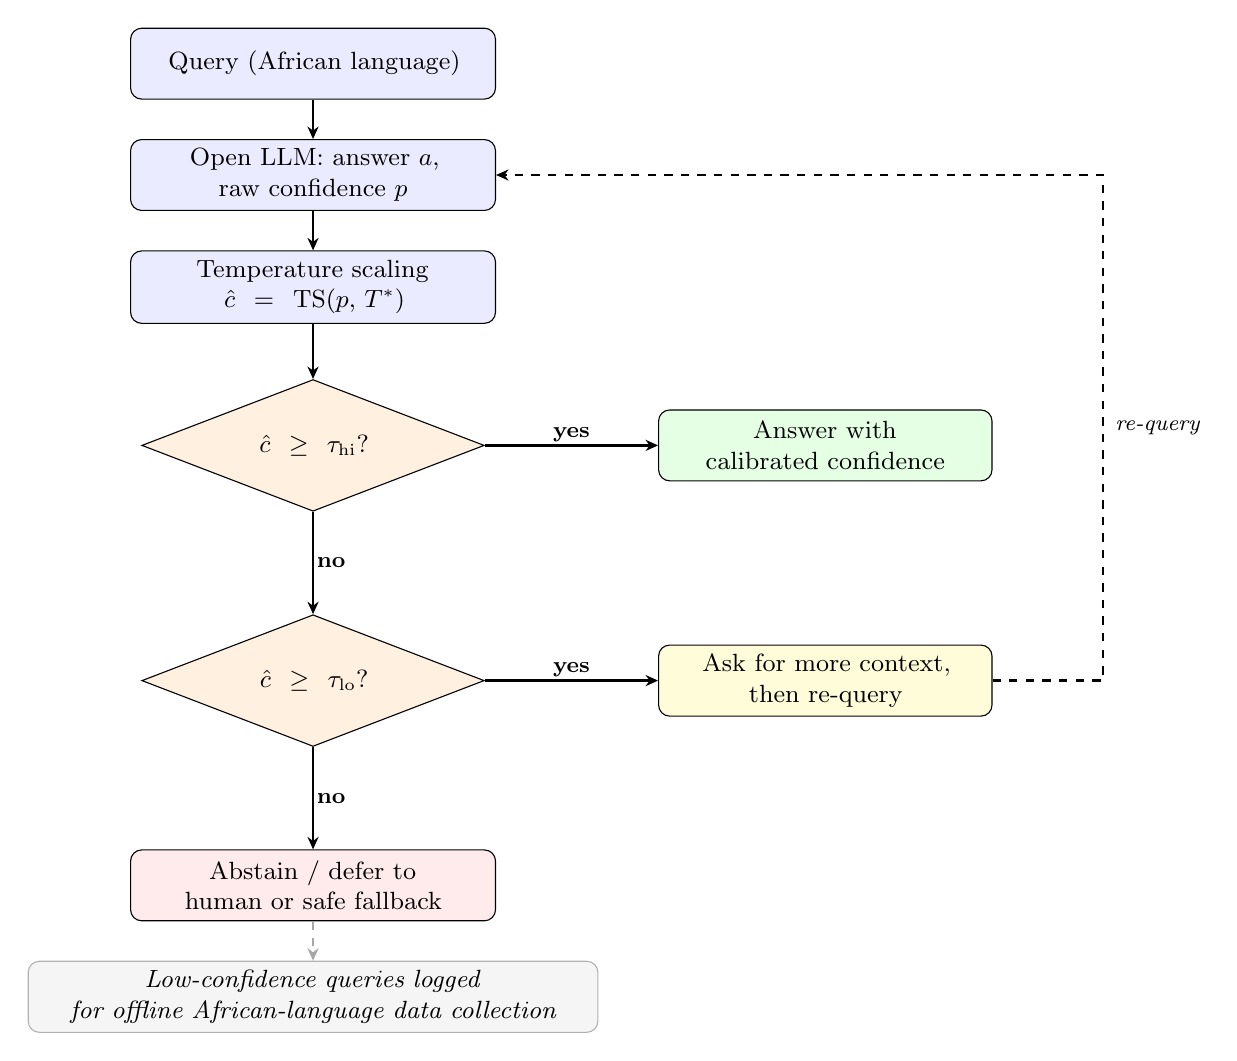
\begin{tikzpicture}[
  node distance  = 5mm,
  every node/.style = {font=\small},
  proc/.style    = {rectangle, rounded corners=4pt, draw, fill=blue!8,
                    text width=44mm, align=center, minimum height=9mm},
  dec/.style     = {diamond, draw, fill=orange!12, aspect=2.6,
                    text width=34mm, align=center, inner sep=1pt},
  outbox/.style  = {rectangle, rounded corners=4pt, draw,
                    text width=40mm, align=center, minimum height=9mm},
  logrect/.style = {rectangle, rounded corners=4pt, draw=gray!60,
                    fill=gray!8, text width=70mm, align=center,
                    minimum height=9mm, font=\small\itshape},
  arr/.style     = {-{Stealth[length=4.5pt,width=4pt]}, thick},
  lbl/.style     = {font=\footnotesize\bfseries, inner sep=1pt},
]

% ── Main vertical spine ──────────────────────────────────────
\node[proc]                   (q)   {Query (African language)};
\node[proc, below=of q]       (llm) {Open LLM: answer $a$,\\ raw confidence $p$};
\node[proc, below=of llm]     (ts)  {Temperature scaling\\ $\hat{c} = \mathrm{TS}(p,\,T^*)$};
\node[dec,  below=7mm of ts]  (d1)  {$\hat{c} \geq \tau_{\mathrm{hi}}$?};
\node[dec,  below=13mm of d1] (d2)  {$\hat{c} \geq \tau_{\mathrm{lo}}$?};
\node[proc, below=13mm of d2, fill=red!8] (abs) {Abstain / defer to\\ human or safe fallback};
\node[logrect, below=5mm of abs] (log) {Low-confidence queries logged\\for offline African-language data collection};

% ── Right-side outcomes ──────────────────────────────────────
\node[outbox, fill=green!10, right=22mm of d1] (ans) {Answer with\\ calibrated confidence};
\node[outbox, fill=yellow!15, right=22mm of d2] (ctx) {Ask for more context,\\ then re-query};

% ── Spine arrows ─────────────────────────────────────────────
\draw[arr] (q)   -- (llm);
\draw[arr] (llm) -- (ts);
\draw[arr] (ts)  -- (d1);
\draw[arr] (d1)  -- node[lbl,right]{no} (d2);
\draw[arr] (d2)  -- node[lbl,right]{no} (abs);
\draw[arr, dashed, gray!70] (abs) -- (log);

% ── Branch arrows ────────────────────────────────────────────
\draw[arr] (d1.east) -- node[lbl,above]{yes} (ans.west);
\draw[arr] (d2.east) -- node[lbl,above]{yes} (ctx.west);

% ── Re-query loop: goes around the RIGHT side, clear of all boxes ──
\draw[arr, dashed]
  (ctx.east)
    -- ++(14mm, 0) coordinate (RightA)
    -- (RightA |- llm.east)  coordinate (RightB)
    -- (llm.east);
\node[font=\footnotesize\itshape, right=1pt] at ($(RightA)!0.5!(RightB)$)
  {re-query};

\end{tikzpicture}
\caption{%
  Deployment framework for LLMs in African languages. Recalibrate first with
  per-language temperature scaling, then route on calibrated confidence $\hat{c}$:
  high values ($\hat{c} \geq \tau_{\mathrm{hi}}$) are answered with the stated
  confidence; medium values trigger a request for more context followed by
  re-query; low values ($\hat{c} < \tau_{\mathrm{lo}}$) are abstained or
  deferred to a human or safe fallback. Thresholds $\tau$ are set per language
  from the risk-coverage curve. Low-confidence queries are logged to drive
  offline African-language data collection.
}
\label{fig:deployment}
\end{figure}

\section{Additional Results}
\label{app:per_lang}

\begin{table}[H]
\centering
\caption{Per-language accuracy and ECE on Uhura-TruthfulQA (zero-shot).
  Each cell shows Acc\,/\,ECE. \textbf{Bold} ECE values exceed the English
  baseline for that model. $\dagger$~OOD for AfroLlama-V1.}
\label{tab:uhura_lang}
\small
\begin{tabular}{lcccc}
\toprule
\textbf{Language} & \textbf{AfroLlama-V1} & \textbf{Aya-Expanse-8B}
                  & \textbf{Gemma-4-12B}  & \textbf{Qwen3-4B} \\
\midrule
English (eng)         & .292\,/\,.177 & .358\,/\,.075 & .329\,/\,.212 & .381\,/\,.072 \\
\midrule
Amharic (amh)$^\dagger$ & .294\,/\,.101 & .302\,/\,.077 & .274\,/\,\textbf{.293} & .373\,/\,.042 \\
Hausa (hau)           & .363\,/\,.085 & .302\,/\,\textbf{.235} & .397\,/\,\textbf{.223} & .308\,/\,\textbf{.199} \\
N.\,Sotho (nso)$^\dagger$ & .246\,/\,\textbf{.307} & .260\,/\,\textbf{.293} & .379\,/\,\textbf{.232} & .270\,/\,\textbf{.262} \\
Swahili (swa)         & .341\,/\,.122 & .314\,/\,\textbf{.215} & .328\,/\,\textbf{.273} & .335\,/\,\textbf{.157} \\
Yoruba (yor)          & .371\,/\,.072 & .351\,/\,\textbf{.141} & .329\,/\,\textbf{.256} & .310\,/\,\textbf{.150} \\
Zulu (zul)            & .337\,/\,.122 & .319\,/\,\textbf{.237} & .343\,/\,\textbf{.266} & .324\,/\,\textbf{.204} \\
\bottomrule
\end{tabular}
\end{table}

\begin{table}[H]
\centering
\caption{Per-language accuracy and ECE on AfriMMLU (zero-shot), representative
  subset of 17 African languages. Each cell shows Acc\,/\,ECE.
  \textbf{Bold} ECE values exceed the English baseline for that model.}
\label{tab:afrimmlu_lang}
\small
\begin{tabular}{lcccc}
\toprule
\textbf{Language} & \textbf{AfroLlama-V1} & \textbf{Aya-Expanse-8B}
                  & \textbf{Gemma-4-12B}  & \textbf{Qwen3-4B} \\
\midrule
English (eng) & .356\,/\,.225 & .520\,/\,.057 & .296\,/\,.311 & .526\,/\,.062 \\
\midrule
Amharic (amh) & .258\,/\,.147 & .240\,/\,\textbf{.114} & .268\,/\,\textbf{.314} & .286\,/\,\textbf{.084} \\
Hausa (hau)   & .294\,/\,.190 & .308\,/\,\textbf{.172} & .308\,/\,\textbf{.309} & .304\,/\,\textbf{.141} \\
Swahili (swa) & .294\,/\,.188 & .312\,/\,\textbf{.151} & .280\,/\,\textbf{.325} & .312\,/\,\textbf{.139} \\
Yoruba (yor)  & .290\,/\,.192 & .300\,/\,\textbf{.154} & .250\,/\,\textbf{.349} & .308\,/\,\textbf{.126} \\
Zulu (zul)    & .310\,/\,.171 & .292\,/\,\textbf{.173} & .252\,/\,\textbf{.362} & .286\,/\,\textbf{.167} \\
Ewe (ewe)     & .244\,/\,\textbf{.239} & .274\,/\,\textbf{.211} & .252\,/\,\textbf{.374} & .288\,/\,\textbf{.175} \\
Igbo (ibo)    & .252\,/\,\textbf{.245} & .262\,/\,\textbf{.214} & .288\,/\,\textbf{.329} & .258\,/\,\textbf{.202} \\
French (fra)  & .280\,/\,\textbf{.268} & .442\,/\,\textbf{.071} & .244\,/\,\textbf{.383} & .372\,/\,\textbf{.114} \\
\bottomrule
\end{tabular}
\end{table}

\begin{table}[H]
\centering
\caption{Per-language temperature scaling on Uhura-TruthfulQA for AfroLlama-V1
  and Qwen3-4B. $T^*$ is selected on the calibration half; ECE values are on
  the held-out half.}
\label{tab:temp_scaling}
\small
\begin{tabular}{l ccc ccc}
\toprule
 & \multicolumn{3}{c}{\textbf{AfroLlama-V1}} & \multicolumn{3}{c}{\textbf{Qwen3-4B}} \\
\cmidrule(lr){2-4}\cmidrule(lr){5-7}
\textbf{Language} & $T^*$ & ECE\textsubscript{bef} & ECE\textsubscript{aft}
                  & $T^*$ & ECE\textsubscript{bef} & ECE\textsubscript{aft} \\
\midrule
English   & 5.0 & .175 & .069 & 1.5 & .096 & .074 \\
Amharic   & 5.0 & .115 & .038 & 1.2 & .056 & .043 \\
Hausa     & 2.0 & .085 & .077 & 5.0 & .203 & .027 \\
N.\,Sotho & 5.0 & .307 & .093 & 5.0 & .260 & .067 \\
Swahili   & 2.0 & .160 & .074 & 3.0 & .182 & .043 \\
Yoruba    & 1.5 & .078 & .064 & 5.0 & .133 & .062 \\
Zulu      & 2.0 & .126 & .046 & 5.0 & .191 & .085 \\
\midrule
\textit{Pooled} & -- & .143 & .036 & -- & .151 & .030 \\
\bottomrule
\end{tabular}
\end{table}

\begin{figure}[H]
\centering
\begin{subfigure}[b]{0.48\textwidth}
  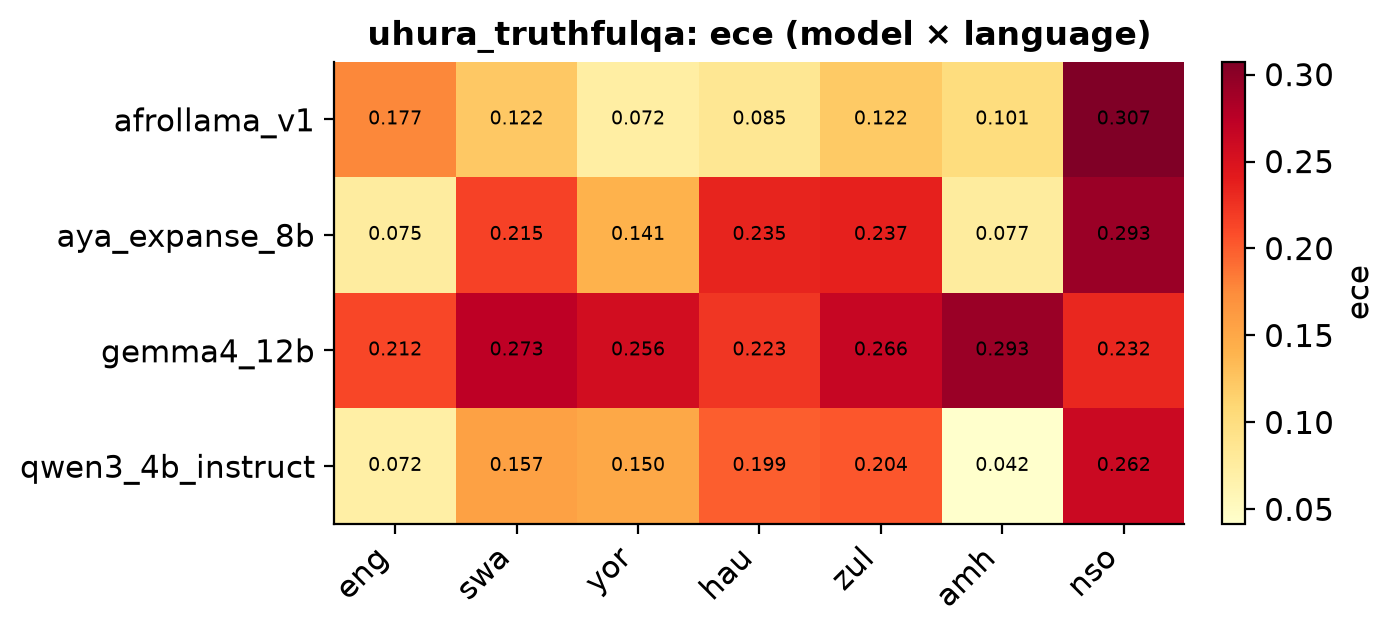
\includegraphics[width=\textwidth]{../artifacts/_comparison/uhura_truthfulqa/ece_heatmap}
  \caption{Uhura-TruthfulQA}
\end{subfigure}
\hfill
\begin{subfigure}[b]{0.48\textwidth}
  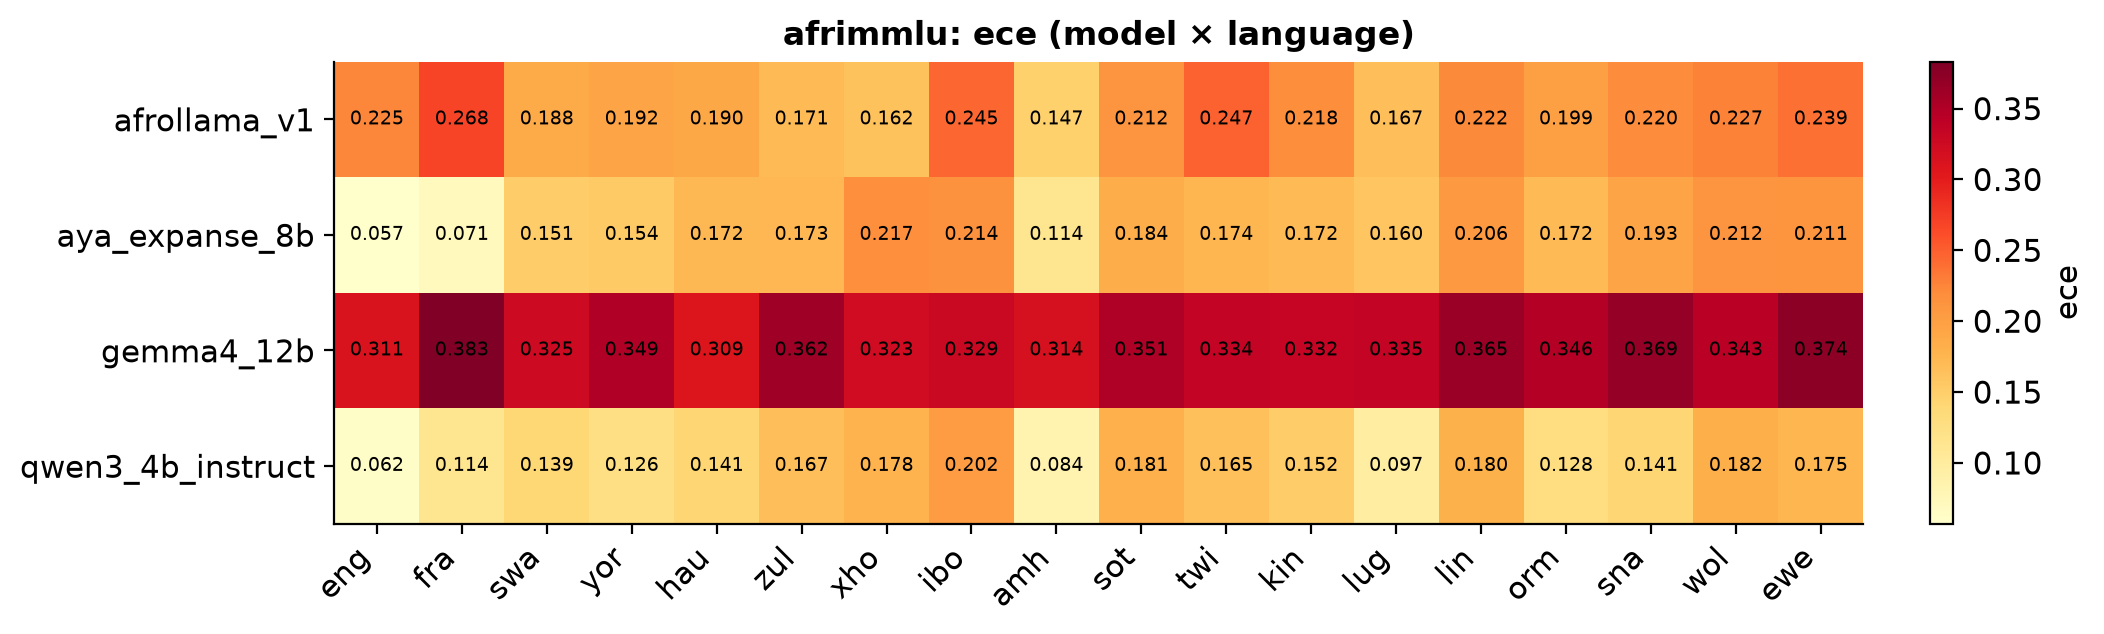
\includegraphics[width=\textwidth]{../artifacts/_comparison/afrimmlu/ece_heatmap}
  \caption{AfriMMLU}
\end{subfigure}
\caption{ECE by model and language. ECE is low in English and rises across
African languages for general-purpose models; AfroLlama-V1 shows the reverse
pattern in its training languages.}
\label{fig:ece_heatmap}
\end{figure}

\begin{figure}[H]
\centering
\begin{subfigure}[b]{0.48\textwidth}
  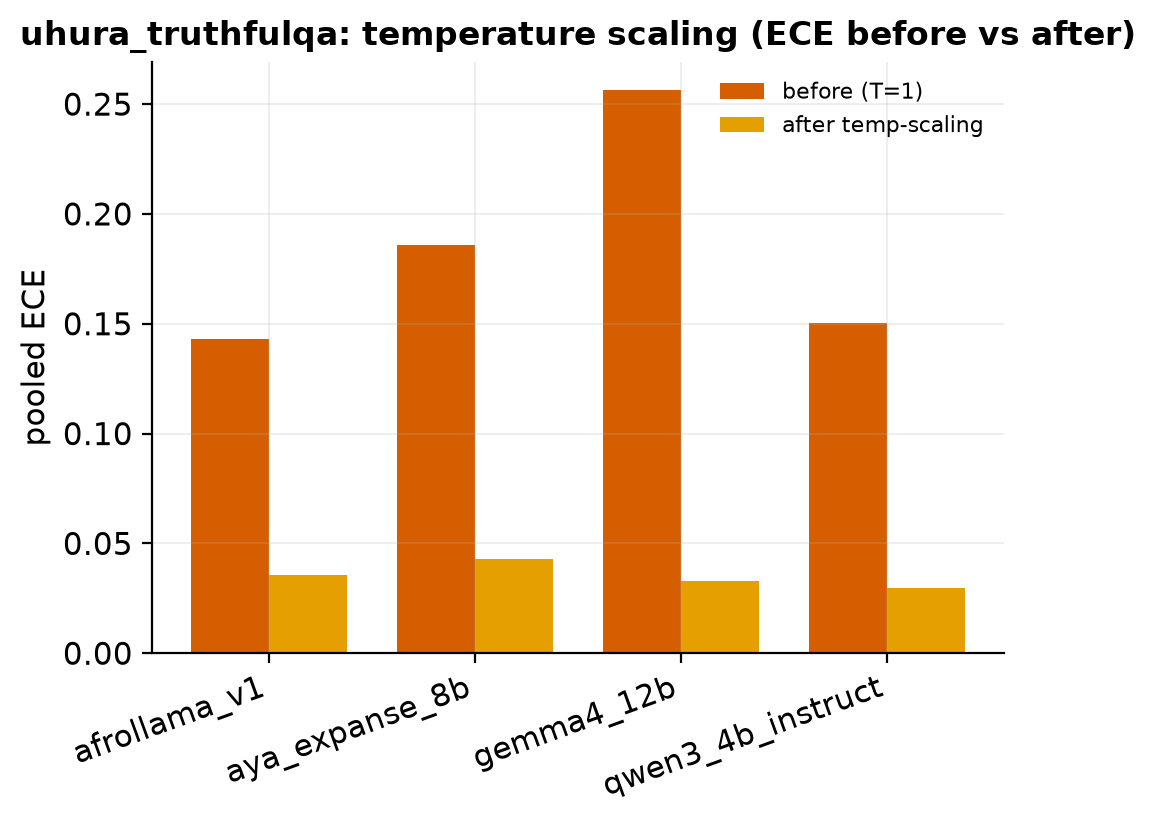
\includegraphics[width=\textwidth]{../artifacts/_comparison/uhura_truthfulqa/temperature_scaling}
  \caption{Uhura-TruthfulQA}
\end{subfigure}
\hfill
\begin{subfigure}[b]{0.48\textwidth}
  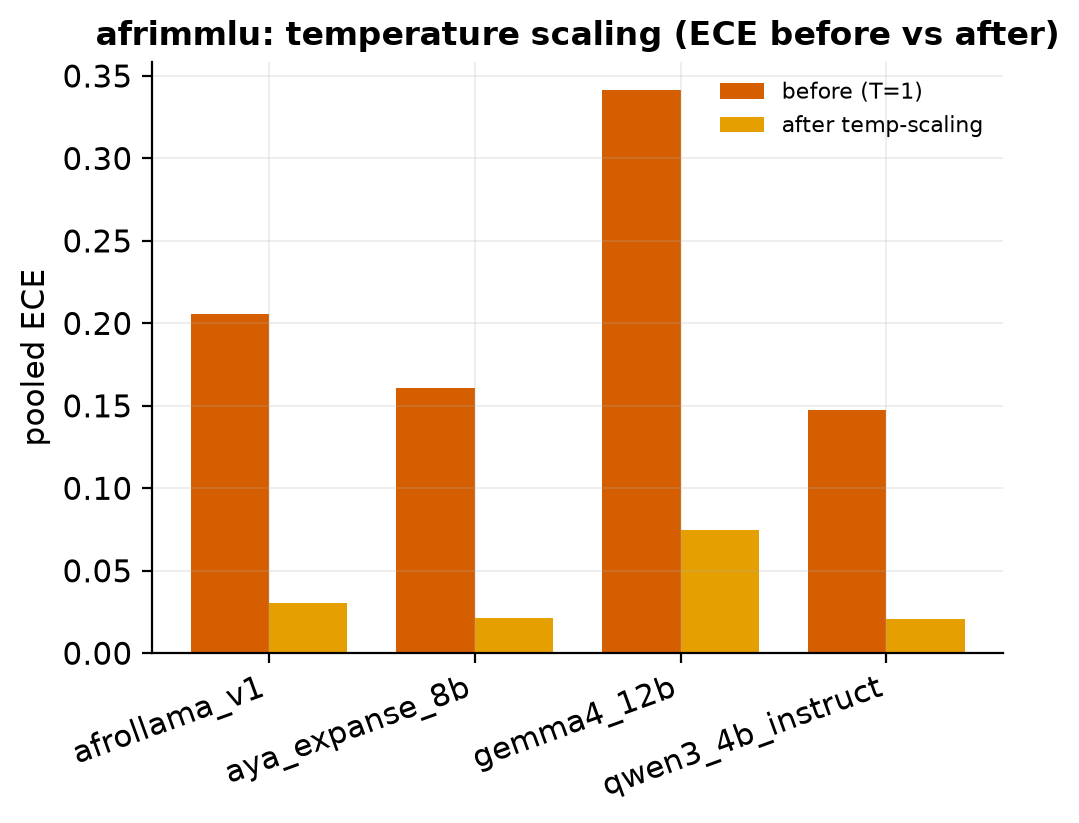
\includegraphics[width=\textwidth]{../artifacts/_comparison/afrimmlu/temperature_scaling}
  \caption{AfriMMLU}
\end{subfigure}
\caption{Pooled ECE before and after per-language temperature scaling.
ECE drops to ${\approx}0.03$ for all models on both datasets.}
\label{fig:temp_scaling}
\end{figure}

\begin{figure}[H]
\centering
\begin{subfigure}[b]{0.48\textwidth}
  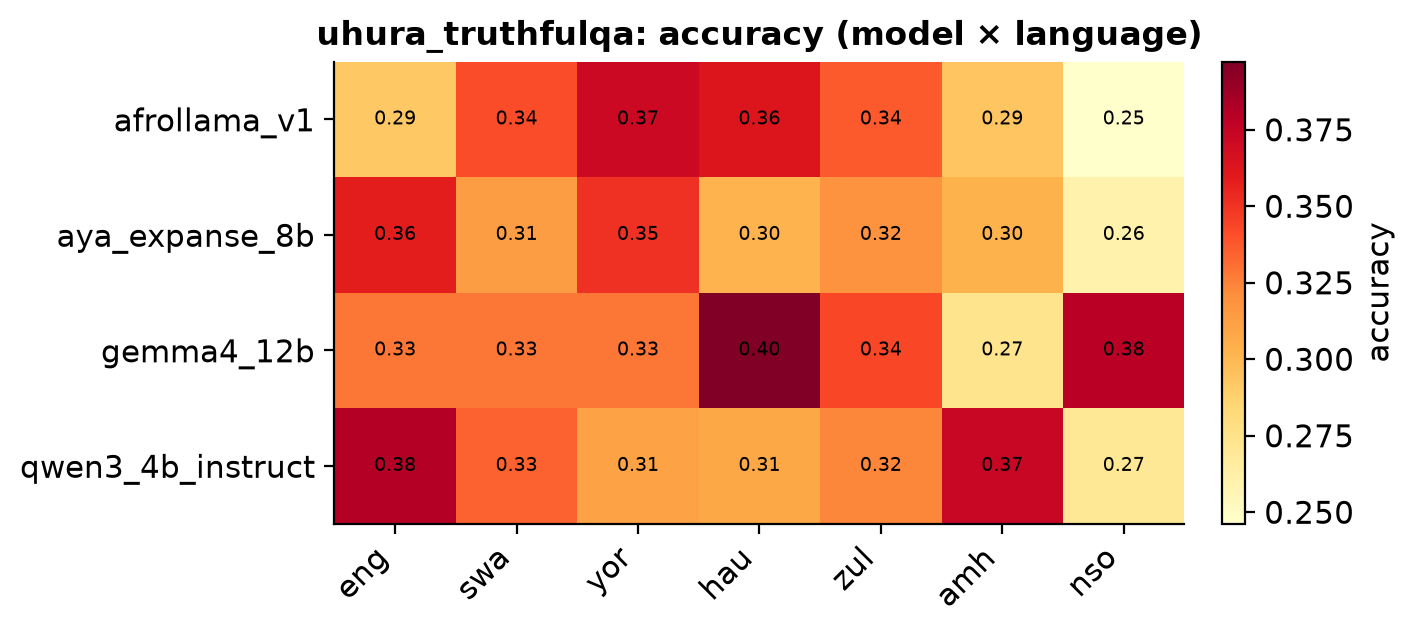
\includegraphics[width=\textwidth]{../artifacts/_comparison/uhura_truthfulqa/accuracy_heatmap}
  \caption{Uhura-TruthfulQA}
\end{subfigure}
\hfill
\begin{subfigure}[b]{0.48\textwidth}
  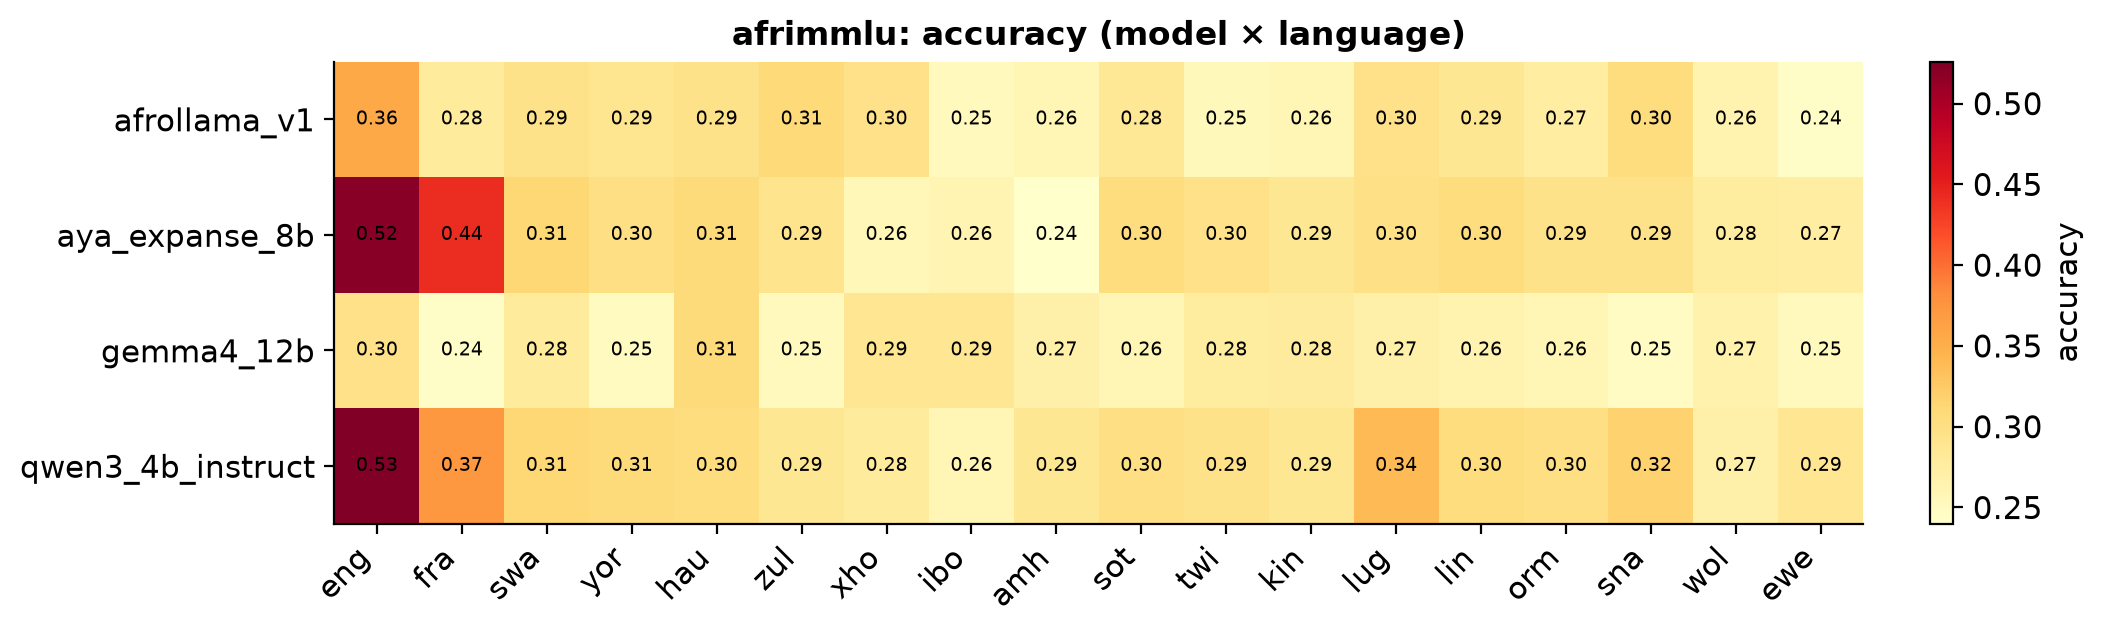
\includegraphics[width=\textwidth]{../artifacts/_comparison/afrimmlu/accuracy_heatmap}
  \caption{AfriMMLU}
\end{subfigure}
\caption{Accuracy by model and language. Long English and French spokes collapse
toward chance across African languages for general-purpose models.}
\label{fig:acc_heatmap}
\end{figure}

\begin{figure}[H]
\centering
\begin{subfigure}[b]{0.48\textwidth}
  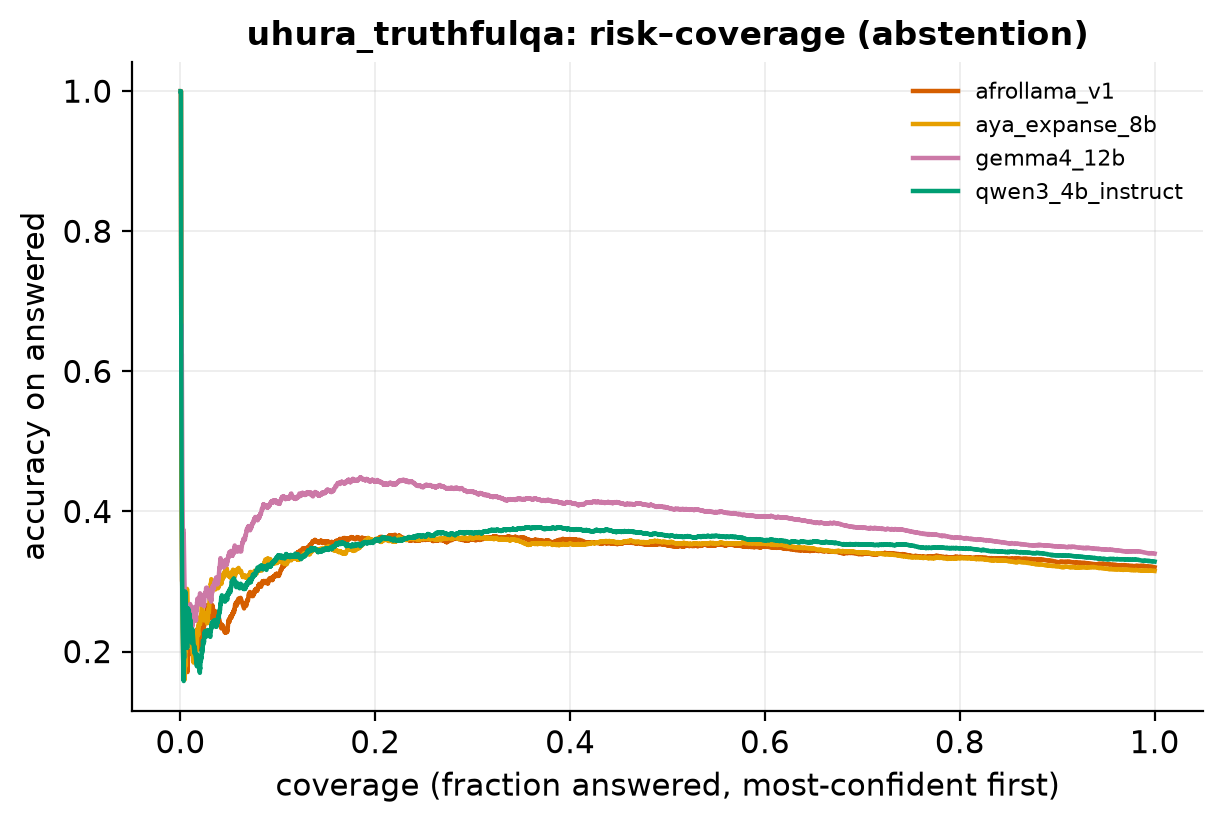
\includegraphics[width=\textwidth]{../artifacts/_comparison/uhura_truthfulqa/risk_coverage}
  \caption{Uhura-TruthfulQA}
\end{subfigure}
\hfill
\begin{subfigure}[b]{0.48\textwidth}
  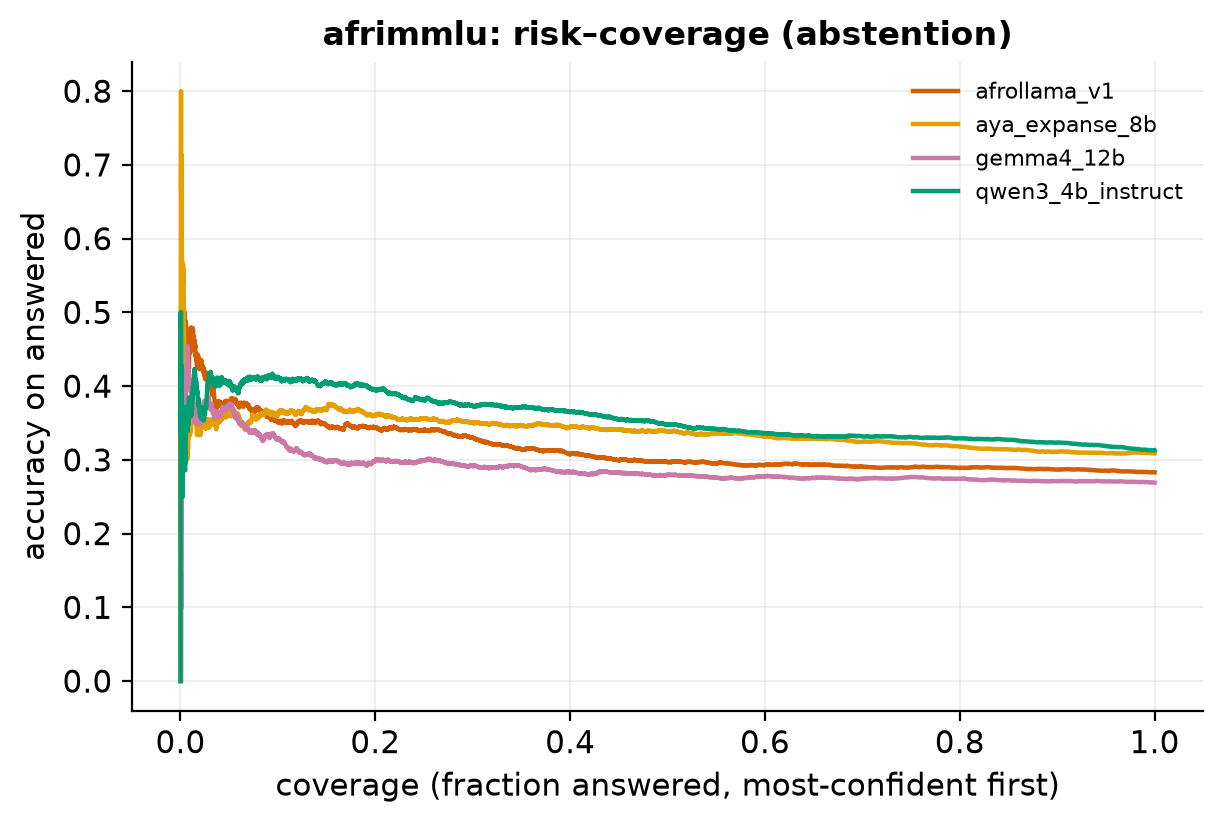
\includegraphics[width=\textwidth]{../artifacts/_comparison/afrimmlu/risk_coverage}
  \caption{AfriMMLU}
\end{subfigure}
\caption{Accuracy-rejection curves under selective abstention. AUARC sits
only modestly above baseline, reflecting a weak uncertainty signal (AUROC
$\approx 0.55$).}
\label{fig:risk_coverage}
\end{figure}

\section{Bootstrap Confidence Intervals}
\label{app:bootstrap}

\Cref{tab:bootstrap_ci} reports 95\% bootstrap confidence intervals (2{,}000
draws, stratified by language, seed~1234) for the four primary point estimates
in \cref{tab:main}. Intervals are computed by resampling within each language
stratum and macro-averaging ECE and accuracy across languages, matching the
aggregation used in the main table.

\begin{table}[H]
\centering
\caption{%
  Bootstrap 95\% confidence intervals for ECE and accuracy in \cref{tab:main}
  (zero-shot, 2{,}000 bootstrap draws, stratified by language, seed~1234).
  Each cell shows point estimate [lower, upper].
}
\label{tab:bootstrap_ci}
\small
\setlength{\tabcolsep}{4pt}
\begin{tabular}{llcccc}
\toprule
\textbf{Model} & \textbf{Dataset}
  & \textbf{ECE\textsubscript{en}}
  & \textbf{ECE\textsubscript{afr}}
  & \textbf{Acc\textsubscript{en}}
  & \textbf{Acc\textsubscript{afr}} \\
\midrule
Qwen3-4B      & Uhura-TQA
  & .072\ [.060,\,.113] & .169\ [.160,\,.186]
  & .381\ [.347,\,.413] & .320\ [.306,\,.333] \\
Gemma-4-12B   & Uhura-TQA
  & .212\ [.182,\,.245] & .257\ [.246,\,.273]
  & .329\ [.297,\,.362] & .342\ [.328,\,.355] \\
Aya-Expanse-8B & Uhura-TQA
  & .075\ [.062,\,.114] & .199\ [.187,\,.214]
  & .358\ [.326,\,.392] & .308\ [.295,\,.321] \\
AfroLlama-V1  & Uhura-TQA
  & .177\ [.148,\,.212] & .135\ [.126,\,.151]
  & .292\ [.261,\,.325] & .325\ [.312,\,.339] \\
\midrule
Qwen3-4B      & AfriMMLU
  & .062\ [.052,\,.116] & .150\ [.147,\,.165]
  & .526\ [.482,\,.572] & .300\ [.290,\,.310] \\
Gemma-4-12B   & AfriMMLU
  & .311\ [.273,\,.354] & .344\ [.335,\,.355]
  & .296\ [.258,\,.336] & .268\ [.259,\,.277] \\
Aya-Expanse-8B & AfriMMLU
  & .057\ [.048,\,.113] & .173\ [.170,\,.189]
  & .520\ [.476,\,.564] & .296\ [.286,\,.306] \\
AfroLlama-V1  & AfriMMLU
  & .225\ [.187,\,.267] & .207\ [.201,\,.219]
  & .356\ [.312,\,.398] & .279\ [.269,\,.288] \\
\bottomrule
\end{tabular}
\end{table}

The English ECE intervals are notably wider than the African-language intervals
because English evaluation is a single-language stratum (no macro-averaging),
while African ECE is macro-averaged over 5--17 languages, which reduces
bootstrap variance. The key qualitative finding---ECE\textsubscript{afr}
consistently exceeds ECE\textsubscript{en} for general-purpose models and is
consistently \emph{lower} for AfroLlama-V1 on Uhura-TQA---is preserved across
the full width of all intervals: the CI for ECE\textsubscript{afr} does not
overlap with the CI for ECE\textsubscript{en} in any general-purpose model row.

\end{document}
